\chapter{Introduction générale}
{\large


Le marché des technologies a connu une énorme évolution ces dernières années et avec
l'intégration de l'internet il y a eu des changements sur la façon et la rapidité d’accès aux
informations. Plusieurs secteurs se sont adaptés à ce changement et encore plus ont vu le
jour pour satisfaire ces nouveaux clients. \\\\
% Le domaine  de couverture social représente l'un des domaines qui connaissent un nombre énorme de citoyen
% et qui souffrent pour les satisfaire. Ils doivent alors proposer leurs services d’une façon
% plus rapide et sécurisé mais aussi à distance,
% afin de pouvoir éviter la congestion dans les
% établissements d'enregistrement social pour le Maroc.
% \\ \\
Avec l’apparition des appareils mobiles, comme les smartphones et les tablettes qui ont
connu une révolution technologique, il est devenu facile pour un établissement de registre social pour le Maroc(CNSS ...) de gérer ce
conflit par proposer une application mobile capable de procurer des services
indispensables rapidement et à tout moment (Interaction avec les citoyens bénéficiaires, notification des citoyens de toute modification dans la situation ...)
.\\ \\Notre projet consiste à développer une application Mobile/Web de register social pour le Maroc  qui
propose de nombreuses fonctionnalités pour le citoyen ainsi que pour l'employé qui peut
consulter et modifier les registres sociaux
 des citoyens facilement.\\ \\
 Le Registre social est un système robuste d’identification et d’enregistrement de la population  ainsi qu’un outil de coordination des programmes d’assistance sociale dans le pays. Il permet d’assurer l’unicité de l’identité et le suivi de l’évolution des conditions socioéconomiques des ménages vulnérables.\\\\
Le rapport de ce projet se divise en  quatre chapitres principaux, le premier est pour détailler l'étude conceptuelle du projet par des  diagrammes d'UML avec  la descriptive de chaque diagramme
, le deuxième un aperçu sur l'ensemble des outils, framework et langages utilisés
  et le troisième chapitre sert des imprimes d'écran de l'application réalisée. Finalement le quatrième chapitre est un rappel de ce qui a été réalisé au niveau de ce projet et les fonctionnalités qui peuvent être ajouté ou amélioré.\\

}
\newpage 
\chapter{Étude générale de projet}
\section{Contexte de projet}
         Dans le Maroc et surtout pour la gestion de registre social on trouve plusieurs employés qui gèrent les travaux des citoyens mais ça nécessite du temps, et la majorité confrontent des difficultés au niveau du déplacement, la perte du temps … .\\\\
         En ces temps de crise, le « ciblage » constitue une pratique primordiale qui vise à promouvoir une croissance et redistribuer la richesse afin de poursuivre des objectifs d’équité sociale. Pour atteindre ces derniers, il faut créer un registre unique permettant d’identifier et de concentrer les services sur les populations les plus nécessiteuses.\\\\ 
       Le domaine de couverture social représente l’un des domaines qui connaissent un nombre énorme de citoyen et qui souffrent pour les satisfaire. Ils doivent alors proposer leurs services d’une façon plus rapide et sécurisé mais aussi à distance, afin de pouvoir éviter la congestion dans les établissements d’enregistrement social pour le Maroc.

% \subsection*{}
% \chapter*{L'objectif de l'application}
% \chapter*{Spécification détaillée}
\section{Spécification détaillée}
\subsection*{}
% {\large
Au cours des dernières années, avec la transformation numérique, l’industrie de la couverture social  a connu des changements majeurs. Un changement évident est la transition des documents papier aux enregistrements numériques par les établissements des regitres sociaux et d’autres installations. \\

Notre application registre social pour le Maroc permet aux employés  d'enregistrer les opérations  des citoyens et aussi les citoyens peuvent consulter leur dossier social et  d’effectuer toutes les opérations
financières. \\\\\\
\subsection*{}
Les fonctionnements de notre application sont :\vspace*{0.5cm}
\begin{itemize}
  \item[$\bullet$] Les principales utilisateurs de l'application sont les citoyens et les employés.\\
  
   \item[$\bullet$] Un employé peut ouvrir un compte d'affiliation à la CNSS.\\
  \item[$\bullet$] Un citoyen peut consulter son dossier social (situation  avec l’organisem de retraite , couverture médicale, …).\\
%   \item[$\bullet$] Un médecin peut apporter des modifications aux dossiers médicaux de ces patients.
  \item[$\bullet$] L'application doit permettre sécuriser et distribuer des données\\

%   \item[$\bullet$] L'application doit permettre le suivie des changements des paramètres vitaux d'un patient donné par son médecin traitant. (Pour l'instant, vous considérez qu'on dispose au préalable des paramètres vitaux des patients).

   \item[$\bullet$]  Les employées doivent être notifier si l'une des opérations financières à effectuer par le citoyen.\\
  \item[$\bullet$]  Les citoyens et les employées doivent s'authentifier pour accéder à l'application.\\
   \item[$\bullet$] L'application Il permet de  contribuer à la simplification des démarches administratives liées aux services fournis aux citoyen
   \\
   \item[$\bullet$] L’application 
 suivie tous les  changements  financières à effectuer par le citoyen.
%   \item[$\bullet$]  Un médecin peut inviter un patient à partager son dossier médical. Puis, le patient accepte ou non le partage de son dossier.
%   \item[$\bullet$]  Pour un diagnostic donné, un médecin peut inviter d'autres médecins collaborateurs pour s'entre-aider à étudier le cas d'un patient donné.
%   \item[$\bullet$]  Pour un diagnostic donné, un médecin peut inviter d'autres médecins collaborateurs pour s'entre-aider à étudier le cas d'un patient donné.
%   \item[$\bullet$] Lorsque un médecin consulte le dossier médical d'un patient, il faut qu'il aie la possibilité de voir seulement les paramètres vitaux d'une (ou plusieurs) maladie(s) donnée(s).

\end{itemize}
\newpage
\subsection*{}
% \chapter*{L'objectif de l'application}
% \chapter*{Spécification détaillée}
% \section{Système existant}
\section{les regitres sociaux existants}
\subsection*{}
\textbf{La sécurité sociale en Suède} [1] : Est  l’une des composantes du système de protection sociale suédois et se compose de diverses assurances sociales gérées par l’Agence nationale d’assurance sociale (suédoise; Försäkringskassan), ainsi que de prestations sociales fournies sur une base de besoins par les municipalités locales. Ils sont les principaux canaux de redistribution d’environ 48\% du PIB suédois sous forme de revenu imposé.  

\begin{figure}[!h]
  \centering
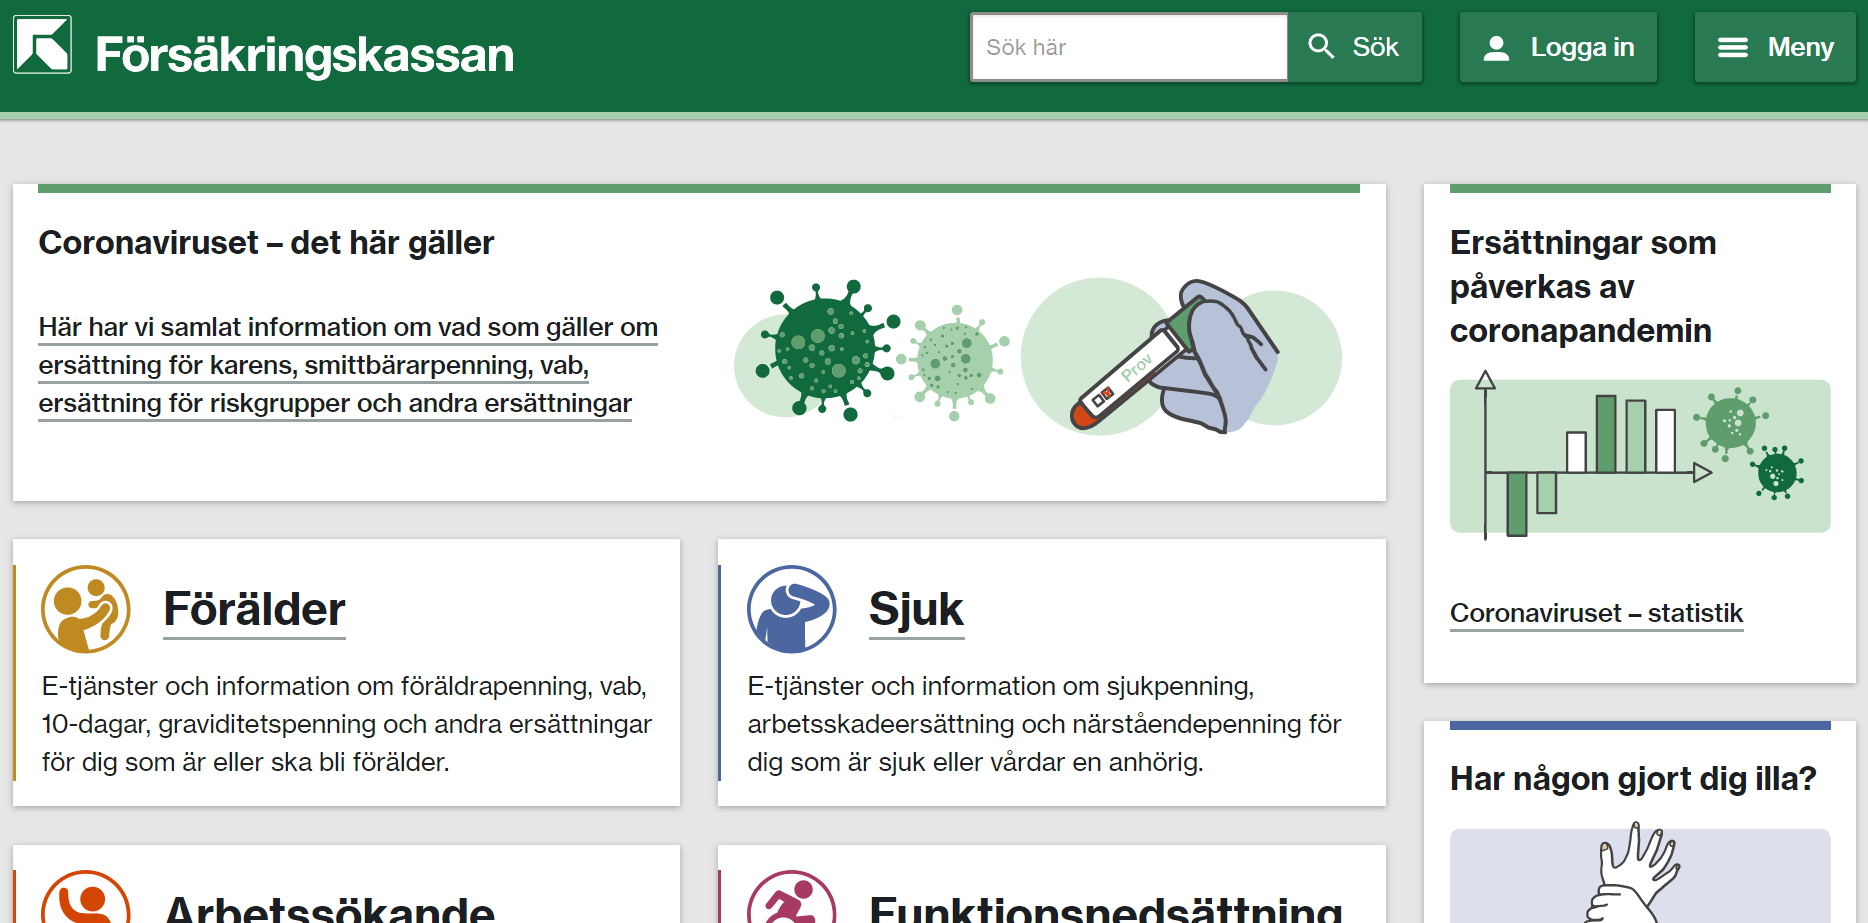
\includegraphics[width=15cm,height=15cm,keepaspectratio]{figure/seq/socity site of sweed.PNG}
  \caption{Site officiel de la sécurité sociale de Suède}
\end{figure}
\\\\

\textbf{La sécurité sociale en États-Unis d'Amérique} [2] : Aux États-Unis, la sécurité sociale est le terme couramment utilisé pour le programme fédéral d’assurance vieillesse, survivants et invalidité (OASDI) et est administré par l’Administration de la sécurité sociale. La première Loi sur la sécurité sociale a été promulguée par Franklin D. Roosevelt en 1935 et la version actuelle de la Loi, telle que modifiée, englobe plusieurs programmes d’aide sociale et d’assurance sociale.\\

\begin{figure}[!h]
  \centering
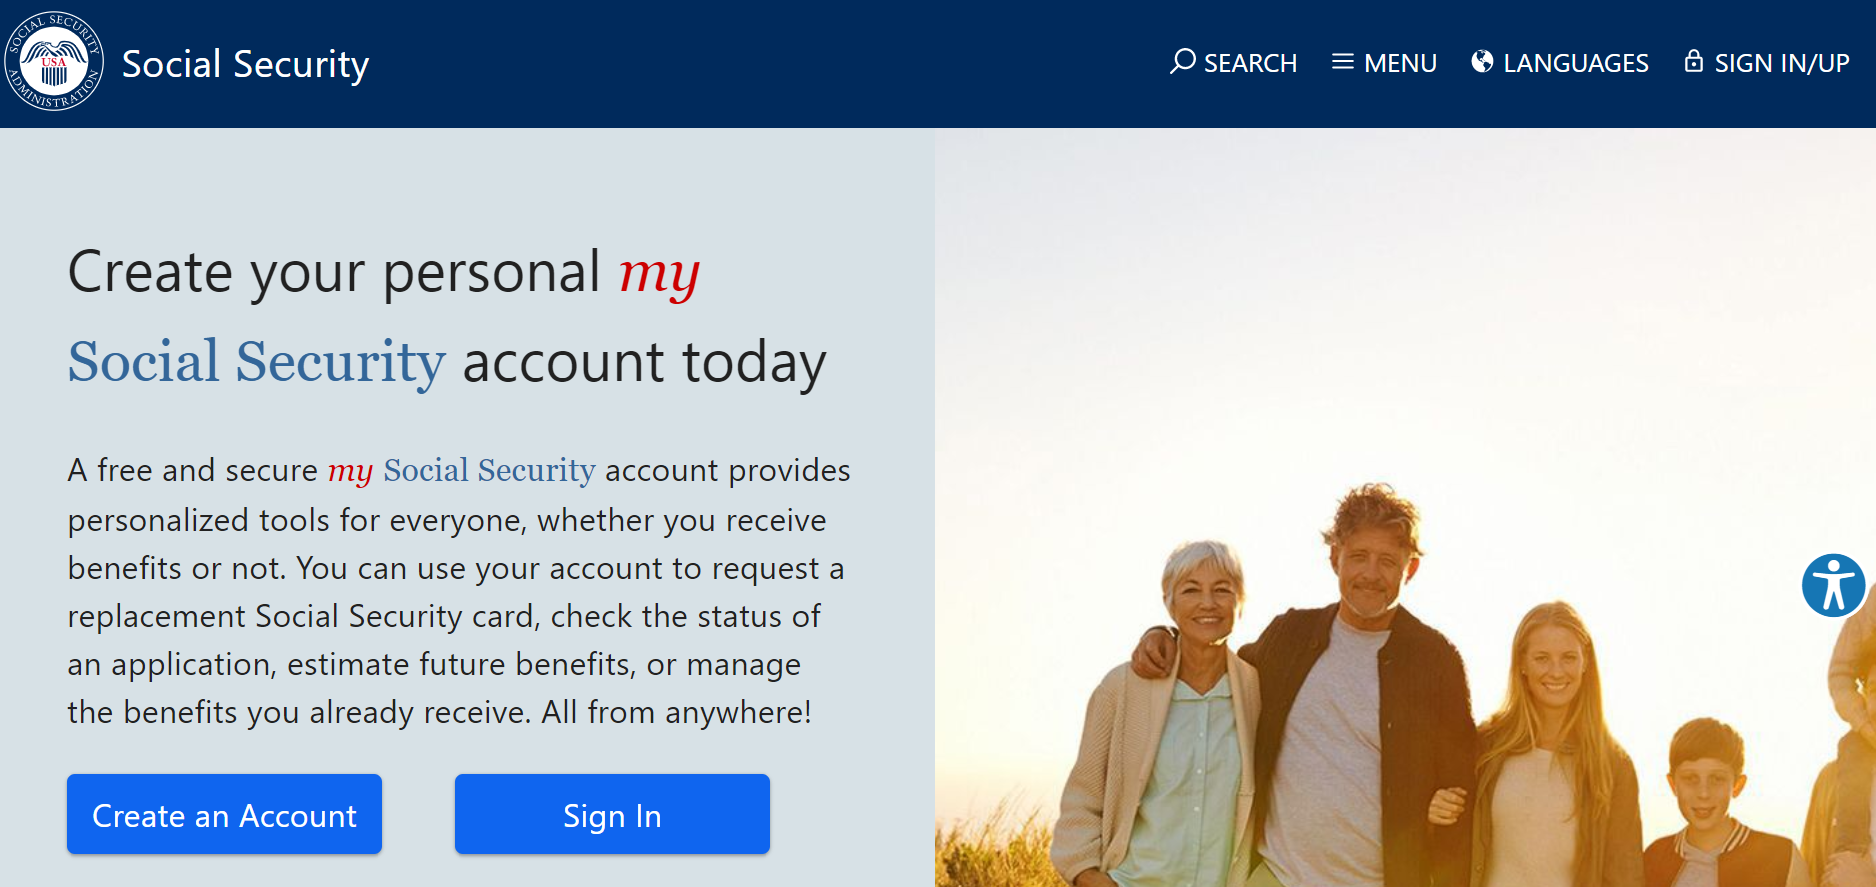
\includegraphics[width=15cm,height=15cm,keepaspectratio]{figure/socity site of america.PNG}
  \caption{Site officiel de la sécurité sociale des États-Unis}
\end{figure}
